\documentclass[]{article}
\usepackage{lmodern}
\usepackage{amssymb,amsmath}
\usepackage{ifxetex,ifluatex}
\usepackage{fixltx2e} % provides \textsubscript
\ifnum 0\ifxetex 1\fi\ifluatex 1\fi=0 % if pdftex
  \usepackage[T1]{fontenc}
  \usepackage[utf8]{inputenc}
\else % if luatex or xelatex
  \ifxetex
    \usepackage{mathspec}
  \else
    \usepackage{fontspec}
  \fi
  \defaultfontfeatures{Ligatures=TeX,Scale=MatchLowercase}
\fi
% use upquote if available, for straight quotes in verbatim environments
\IfFileExists{upquote.sty}{\usepackage{upquote}}{}
% use microtype if available
\IfFileExists{microtype.sty}{%
\usepackage{microtype}
\UseMicrotypeSet[protrusion]{basicmath} % disable protrusion for tt fonts
}{}
\usepackage[margin=1in]{geometry}
\usepackage{hyperref}
\hypersetup{unicode=true,
            pdftitle={Final Project},
            pdfauthor={Christophe Hunt},
            pdfborder={0 0 0},
            breaklinks=true}
\urlstyle{same}  % don't use monospace font for urls
\usepackage{color}
\usepackage{fancyvrb}
\newcommand{\VerbBar}{|}
\newcommand{\VERB}{\Verb[commandchars=\\\{\}]}
\DefineVerbatimEnvironment{Highlighting}{Verbatim}{commandchars=\\\{\}}
% Add ',fontsize=\small' for more characters per line
\usepackage{framed}
\definecolor{shadecolor}{RGB}{248,248,248}
\newenvironment{Shaded}{\begin{snugshade}}{\end{snugshade}}
\newcommand{\KeywordTok}[1]{\textcolor[rgb]{0.13,0.29,0.53}{\textbf{{#1}}}}
\newcommand{\DataTypeTok}[1]{\textcolor[rgb]{0.13,0.29,0.53}{{#1}}}
\newcommand{\DecValTok}[1]{\textcolor[rgb]{0.00,0.00,0.81}{{#1}}}
\newcommand{\BaseNTok}[1]{\textcolor[rgb]{0.00,0.00,0.81}{{#1}}}
\newcommand{\FloatTok}[1]{\textcolor[rgb]{0.00,0.00,0.81}{{#1}}}
\newcommand{\ConstantTok}[1]{\textcolor[rgb]{0.00,0.00,0.00}{{#1}}}
\newcommand{\CharTok}[1]{\textcolor[rgb]{0.31,0.60,0.02}{{#1}}}
\newcommand{\SpecialCharTok}[1]{\textcolor[rgb]{0.00,0.00,0.00}{{#1}}}
\newcommand{\StringTok}[1]{\textcolor[rgb]{0.31,0.60,0.02}{{#1}}}
\newcommand{\VerbatimStringTok}[1]{\textcolor[rgb]{0.31,0.60,0.02}{{#1}}}
\newcommand{\SpecialStringTok}[1]{\textcolor[rgb]{0.31,0.60,0.02}{{#1}}}
\newcommand{\ImportTok}[1]{{#1}}
\newcommand{\CommentTok}[1]{\textcolor[rgb]{0.56,0.35,0.01}{\textit{{#1}}}}
\newcommand{\DocumentationTok}[1]{\textcolor[rgb]{0.56,0.35,0.01}{\textbf{\textit{{#1}}}}}
\newcommand{\AnnotationTok}[1]{\textcolor[rgb]{0.56,0.35,0.01}{\textbf{\textit{{#1}}}}}
\newcommand{\CommentVarTok}[1]{\textcolor[rgb]{0.56,0.35,0.01}{\textbf{\textit{{#1}}}}}
\newcommand{\OtherTok}[1]{\textcolor[rgb]{0.56,0.35,0.01}{{#1}}}
\newcommand{\FunctionTok}[1]{\textcolor[rgb]{0.00,0.00,0.00}{{#1}}}
\newcommand{\VariableTok}[1]{\textcolor[rgb]{0.00,0.00,0.00}{{#1}}}
\newcommand{\ControlFlowTok}[1]{\textcolor[rgb]{0.13,0.29,0.53}{\textbf{{#1}}}}
\newcommand{\OperatorTok}[1]{\textcolor[rgb]{0.81,0.36,0.00}{\textbf{{#1}}}}
\newcommand{\BuiltInTok}[1]{{#1}}
\newcommand{\ExtensionTok}[1]{{#1}}
\newcommand{\PreprocessorTok}[1]{\textcolor[rgb]{0.56,0.35,0.01}{\textit{{#1}}}}
\newcommand{\AttributeTok}[1]{\textcolor[rgb]{0.77,0.63,0.00}{{#1}}}
\newcommand{\RegionMarkerTok}[1]{{#1}}
\newcommand{\InformationTok}[1]{\textcolor[rgb]{0.56,0.35,0.01}{\textbf{\textit{{#1}}}}}
\newcommand{\WarningTok}[1]{\textcolor[rgb]{0.56,0.35,0.01}{\textbf{\textit{{#1}}}}}
\newcommand{\AlertTok}[1]{\textcolor[rgb]{0.94,0.16,0.16}{{#1}}}
\newcommand{\ErrorTok}[1]{\textcolor[rgb]{0.64,0.00,0.00}{\textbf{{#1}}}}
\newcommand{\NormalTok}[1]{{#1}}
\usepackage{longtable,booktabs}
\usepackage{graphicx,grffile}
\makeatletter
\def\maxwidth{\ifdim\Gin@nat@width>\linewidth\linewidth\else\Gin@nat@width\fi}
\def\maxheight{\ifdim\Gin@nat@height>\textheight\textheight\else\Gin@nat@height\fi}
\makeatother
% Scale images if necessary, so that they will not overflow the page
% margins by default, and it is still possible to overwrite the defaults
% using explicit options in \includegraphics[width, height, ...]{}
\setkeys{Gin}{width=\maxwidth,height=\maxheight,keepaspectratio}
\IfFileExists{parskip.sty}{%
\usepackage{parskip}
}{% else
\setlength{\parindent}{0pt}
\setlength{\parskip}{6pt plus 2pt minus 1pt}
}
\setlength{\emergencystretch}{3em}  % prevent overfull lines
\providecommand{\tightlist}{%
  \setlength{\itemsep}{0pt}\setlength{\parskip}{0pt}}
\setcounter{secnumdepth}{5}
% Redefines (sub)paragraphs to behave more like sections
\ifx\paragraph\undefined\else
\let\oldparagraph\paragraph
\renewcommand{\paragraph}[1]{\oldparagraph{#1}\mbox{}}
\fi
\ifx\subparagraph\undefined\else
\let\oldsubparagraph\subparagraph
\renewcommand{\subparagraph}[1]{\oldsubparagraph{#1}\mbox{}}
\fi

%%% Use protect on footnotes to avoid problems with footnotes in titles
\let\rmarkdownfootnote\footnote%
\def\footnote{\protect\rmarkdownfootnote}

%%% Change title format to be more compact
\usepackage{titling}

% Create subtitle command for use in maketitle
\newcommand{\subtitle}[1]{
  \posttitle{
    \begin{center}\large#1\end{center}
    }
}

\setlength{\droptitle}{-2em}
  \title{Final Project}
  \pretitle{\vspace{\droptitle}\centering\huge}
  \posttitle{\par}
  \author{Christophe Hunt}
  \preauthor{\centering\large\emph}
  \postauthor{\par}
  \predate{\centering\large\emph}
  \postdate{\par}
  \date{May 13, 2017}

\usepackage{relsize}
\usepackage{setspace}
\usepackage{amsmath,amsfonts,amsthm}
\usepackage[sfdefault]{roboto}
\usepackage[T1]{fontenc}
\usepackage{float}
\usepackage{multirow}
\usepackage{mathtools}
\usepackage{tikz}
\usepackage{ragged2e}

% https://github.com/jacbar/studia/blob/master/semestr-vii/inz-tymon/main/header.pandoc#L10
\usepackage{lscape}
\usepackage{pdfpages}
\usepackage{geometry}

% pandoc does not parse latex env - https://groups.google.com/forum/?fromgroups=#!topic/pandoc-discuss/oZETB5Ii1Cw
\newcommand{\blandscape}{\begin{landscape}}
\newcommand{\elandscape}{\end{landscape}}

\begin{document}
\maketitle

{
\setcounter{tocdepth}{2}
\tableofcontents
}
Pick one of the quantitative independent variables from the training
data set (train.csv), and define that variable as X.

Pick SalePrice as the dependent variable, and define it as Y for the
next analysis.

\begin{Shaded}
\begin{Highlighting}[]
\KeywordTok{library}\NormalTok{(tidyverse)}
\NormalTok{train.df <-}\StringTok{ }\KeywordTok{as_tibble}\NormalTok{(}\KeywordTok{read.csv}\NormalTok{(}\StringTok{"https://raw.githubusercontent.com/ChristopheHunt/MSDA---Coursework/master/Data%20605/Final%20Project/train.csv"}\NormalTok{))}
\end{Highlighting}
\end{Shaded}

\begin{Shaded}
\begin{Highlighting}[]
\NormalTok{sub.train.df <-}\StringTok{ }\NormalTok{train.df[, }\KeywordTok{c}\NormalTok{(}\StringTok{"SalePrice"}\NormalTok{, }\StringTok{"LotArea"}\NormalTok{)]}
\end{Highlighting}
\end{Shaded}

\begin{quote}
The variable we will set to X is LotArea, which is defined as the Lot
size in square feet. I chose this because an anecdotal assumption is
that the larger the lot size is the higher the sale price. However,
living in NYC there are tiny lots in very desirable places that have a
high price so I believe there may be some interesting patterns here.
\end{quote}

\section{Probability}\label{probability}

Calculate as a minimum the below probabilities a through c.

Assume the small letter ``x'' is estimated as the 4th quartile of the X
variable, and the small letter ``y'' is estimated as the 2nd quartile of
the Y variable. Interpret the meaning of all probabilities.

\begin{enumerate}
\def\labelenumi{\alph{enumi}.}
\tightlist
\item
  \(P(X>x | Y>y)\)
\end{enumerate}

\begin{Shaded}
\begin{Highlighting}[]
\NormalTok{prob.x <-}\StringTok{ }\KeywordTok{list}\NormalTok{(}\DataTypeTok{qrtx =} \KeywordTok{as.numeric}\NormalTok{(}\KeywordTok{quantile}\NormalTok{(sub.train.df$LotArea)[}\DecValTok{4}\NormalTok{]), }
               \DataTypeTok{mean =} \KeywordTok{mean}\NormalTok{(sub.train.df$LotArea), }
               \DataTypeTok{std =} \KeywordTok{sd}\NormalTok{(sub.train.df$LotArea))}

\NormalTok{prob.y <-}\StringTok{ }\KeywordTok{list}\NormalTok{(}\DataTypeTok{qrtx =} \KeywordTok{as.numeric}\NormalTok{(}\KeywordTok{quantile}\NormalTok{(sub.train.df$SalePrice)[}\DecValTok{2}\NormalTok{]), }
               \DataTypeTok{mean =} \KeywordTok{mean}\NormalTok{(sub.train.df$SalePrice), }
               \DataTypeTok{std =} \KeywordTok{sd}\NormalTok{(sub.train.df$SalePrice))}
\end{Highlighting}
\end{Shaded}

\begin{enumerate}
\def\labelenumi{\alph{enumi}.}
\setcounter{enumi}{1}
\item
  \(P(X>x, Y>y)\)
\item
  \(P(X<x | Y>y)\)
\end{enumerate}

Does splitting the training data in this fashion make them independent?

In other words, does \(P(X|Y)=P(X)P(Y))\)?

Check mathematically, and then evaluate by running a Chi Square test for
association.

You might have to research this.

\section{Descriptive and Inferential
Statistics.}\label{descriptive-and-inferential-statistics.}

Provide univariate descriptive statistics and appropriate plots for both
variables.

Provide a scatterplot of X and Y.

\begin{Shaded}
\begin{Highlighting}[]
\KeywordTok{ggplot}\NormalTok{(sub.train.df, }\KeywordTok{aes}\NormalTok{(}\DataTypeTok{x =} \NormalTok{LotArea, }\DataTypeTok{y =} \NormalTok{SalePrice)) +}\StringTok{ }\KeywordTok{geom_point}\NormalTok{(}\DataTypeTok{shape =} \DecValTok{1}\NormalTok{) +}\StringTok{ }
\StringTok{    }\KeywordTok{theme_light}\NormalTok{() +}\StringTok{ }\KeywordTok{scale_y_continuous}\NormalTok{(}\DataTypeTok{labels =} \NormalTok{dollar)}
\end{Highlighting}
\end{Shaded}

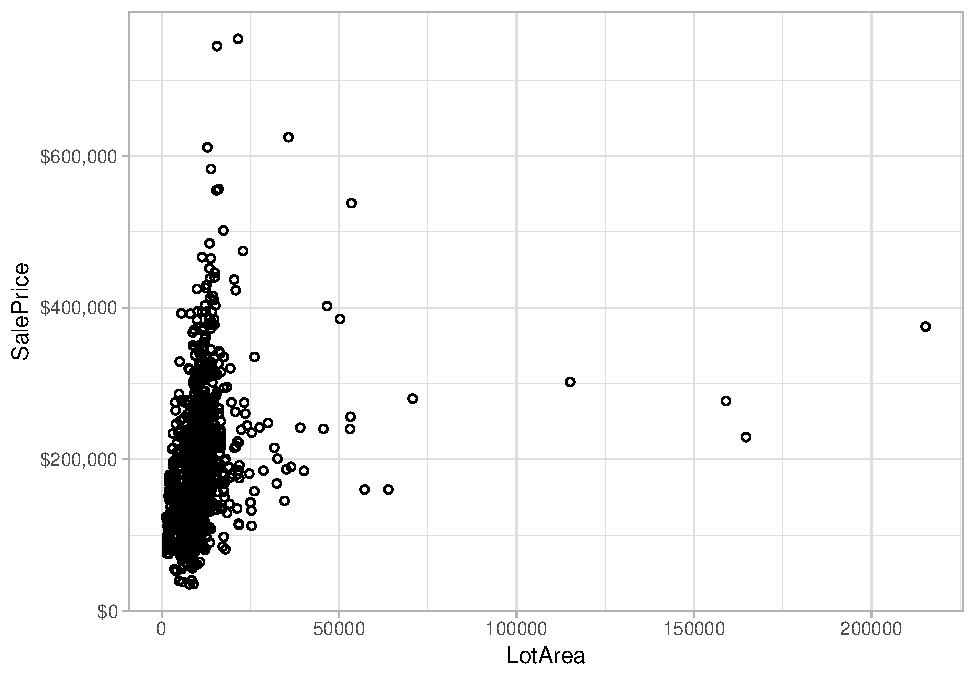
\includegraphics{Final_Project_files/figure-latex/scatter plot-1.pdf}

Transform both variables simultaneously using Box-Cox transformations.

\begin{quote}
I am using the \texttt{BoxCox.lambda} function from the
\texttt{forecast} package to determine the necessary transformations for
the two variables.
\end{quote}

\begin{Shaded}
\begin{Highlighting}[]
\KeywordTok{library}\NormalTok{(forecast)}
\KeywordTok{library}\NormalTok{(knitr)}
\NormalTok{l1 <-}\StringTok{ }\KeywordTok{BoxCox.lambda}\NormalTok{(}\KeywordTok{as.numeric}\NormalTok{(sub.train.df$SalePrice))}
\NormalTok{l2 <-}\StringTok{ }\KeywordTok{BoxCox.lambda}\NormalTok{(}\KeywordTok{as.numeric}\NormalTok{(sub.train.df$LotArea))}

\NormalTok{lamdas <-}\StringTok{ }\KeywordTok{c}\NormalTok{(l1, l2)}
\NormalTok{Variables <-}\StringTok{ }\KeywordTok{c}\NormalTok{(}\StringTok{"SalePrice"}\NormalTok{, }\StringTok{"LotArea"}\NormalTok{)}
\NormalTok{dfBoxCox <-}\StringTok{ }\KeywordTok{as.data.frame}\NormalTok{(}\KeywordTok{cbind}\NormalTok{(}\KeywordTok{round}\NormalTok{(}\KeywordTok{as.numeric}\NormalTok{(lamdas),}\DecValTok{4}\NormalTok{), Variables))}
\KeywordTok{colnames}\NormalTok{(dfBoxCox) <-}\StringTok{ }\KeywordTok{c}\NormalTok{(}\StringTok{"$}\CharTok{\textbackslash{}\textbackslash{}}\StringTok{lambda$"}\NormalTok{, }\StringTok{"Variables"}\NormalTok{)}
\KeywordTok{kable}\NormalTok{(dfBoxCox, }\DataTypeTok{align =} \KeywordTok{c}\NormalTok{(}\StringTok{"c"}\NormalTok{, }\StringTok{"c"}\NormalTok{))}
\end{Highlighting}
\end{Shaded}

\begin{longtable}[]{@{}cc@{}}
\toprule
\(\lambda\) & Variables\tabularnewline
\midrule
\endhead
-0.3308 & SalePrice\tabularnewline
-0.1268 & LotArea\tabularnewline
\bottomrule
\end{longtable}

\centering

Common Box-Cox Transformations\footnote{Osborne, Jason W. ``Improving
  your data transformations: Applying the Box-Cox transformation.''
  Practical Assessment, Research \& Evaluation 15.12 (2010): 1-9.}
\footnote{\href{https://www.isixsigma.com/tools-templates/normality/making-data-normal-using-box-cox-power-transformation/}{By
  Understanding Both the Concept of Transformation and the Box-Cox
  Method, Practitioners Will Be Better Prepared to Work with Non-normal
  Data.} . ``Making Data Normal Using Box-Cox Power Transformation.''
  ISixSigma. N.p., n.d. Web. 29 Oct. 2016.}

\setlength{\tabcolsep}{12pt}

\begin{tabular}{ c c }
\hline
$\lambda$ & Y' \\ \hline
-0.5 &  $Y^{-0.5}~=~\frac{1}{\sqrt{(Y)}}$ \\
0   & $\log(Y)$ \\
.25  & $\sqrt[4]{Y}$
\end{tabular}

\justifying

Lambda values were truncated to the nearest tenth that match a common
transformation as per the below table.

\centering

\begin{tabular}{ c c }
\hline
variable & variable transformation \\ \hline
SalePrice & $SalePrice^{-0.5}$ \\
LotArea & $log(LotArea)$ 
\end{tabular}

\justifying

\setlength{\tabcolsep}{6pt}

\subsection{TODO Expand on the correlation
analysis}\label{todo-expand-on-the-correlation-analysis}

Using the transformed variables, run a correlation analysis and
interpret.

\begin{Shaded}
\begin{Highlighting}[]
\NormalTok{sub.train.df.trans <-}\StringTok{ }\NormalTok{sub.train.df %>%}\StringTok{ }
\StringTok{                      }\KeywordTok{mutate}\NormalTok{(}\DataTypeTok{SalePrice =} \NormalTok{SalePrice^(-.}\DecValTok{5}\NormalTok{), }
                             \DataTypeTok{LotArea =} \KeywordTok{log}\NormalTok{(LotArea))}

\NormalTok{sub.train.cor <-}\StringTok{ }\KeywordTok{cor.test}\NormalTok{(sub.train.df.trans$SalePrice, }
                          \NormalTok{sub.train.df.trans$LotArea, }
                          \DataTypeTok{method =} \StringTok{"pearson"}\NormalTok{, }\DataTypeTok{conf.level =} \NormalTok{.}\DecValTok{99}\NormalTok{)}
\NormalTok{sub.train.cor}
\end{Highlighting}
\end{Shaded}

\begin{verbatim}
## 
##  Pearson's product-moment correlation
## 
## data:  sub.train.df.trans$SalePrice and sub.train.df.trans$LotArea
## t = -15.968, df = 1458, p-value < 2.2e-16
## alternative hypothesis: true correlation is not equal to 0
## 99 percent confidence interval:
##  -0.4417063 -0.3269282
## sample estimates:
##        cor 
## -0.3858091
\end{verbatim}

\begin{quote}
The p-value of the correlation test is 2.2e-16 which is less than the
significance level of alpha at .05. We are using the standard alpha as
there is no indication another any other value for alpha should be used.
We can therefore say that the log of lot size and sale price raised to
the -.5 power are significantly correlated with a negative correlation
coefficient of -0.386.
\end{quote}

Test the hypothesis that the correlation between these variables is 0
and provide a 99\% confidence interval.

\begin{quote}
The correlation test has specifically done that for us and we can safely
reject the null hypothesis as we see that our 99\% confidence interval
exists at the values (-0.441, -0.327) with a p-value \textless{}
2.2e-16.
\end{quote}

Discuss the meaning of your analysis.

\begin{quote}
This means two possible things could have occured, there is no
correlation and this data set is pulled from an unusual set of house
sales. Or, more likely with the values obtained, our assumption of 0
correlation is incorect and we have obtained a very typical data set and
must reject the null hypothesis because correlation does exist.
\end{quote}

\section{Linear Algebra and
Correlation.}\label{linear-algebra-and-correlation.}

\begin{Shaded}
\begin{Highlighting}[]
\NormalTok{A <-}\StringTok{ }\KeywordTok{cor}\NormalTok{(sub.train.df.trans)}
\KeywordTok{kable}\NormalTok{(A)}
\end{Highlighting}
\end{Shaded}

\begin{longtable}[]{@{}lrr@{}}
\toprule
& SalePrice & LotArea\tabularnewline
\midrule
\endhead
SalePrice & 1.0000000 & -0.3858091\tabularnewline
LotArea & -0.3858091 & 1.0000000\tabularnewline
\bottomrule
\end{longtable}

Invert your correlation matrix.(This is known as the precision matrix
and contains variance inflation factors on the diagonal.)

\begin{Shaded}
\begin{Highlighting}[]
\NormalTok{B <-}\StringTok{ }\KeywordTok{solve}\NormalTok{(A)}
\KeywordTok{kable}\NormalTok{(B)}
\end{Highlighting}
\end{Shaded}

\begin{longtable}[]{@{}lrr@{}}
\toprule
& SalePrice & LotArea\tabularnewline
\midrule
\endhead
SalePrice & 1.1748792 & 0.4532792\tabularnewline
LotArea & 0.4532792 & 1.1748792\tabularnewline
\bottomrule
\end{longtable}

Multiply the correlation matrix by the precision matrix, and then
multiply the precision matrix by the correlation matrix.

\begin{Shaded}
\begin{Highlighting}[]
\NormalTok{corr.by.pre.M <-}\StringTok{ }\NormalTok{A %*%}\StringTok{ }\NormalTok{B}
\KeywordTok{kable}\NormalTok{(corr.by.pre.M)}
\end{Highlighting}
\end{Shaded}

\begin{longtable}[]{@{}lrr@{}}
\toprule
& SalePrice & LotArea\tabularnewline
\midrule
\endhead
SalePrice & 1 & 0\tabularnewline
LotArea & 0 & 1\tabularnewline
\bottomrule
\end{longtable}

\begin{Shaded}
\begin{Highlighting}[]
\NormalTok{pre.by.corr.M <-}\StringTok{ }\NormalTok{B %*%}\StringTok{ }\NormalTok{A}
\KeywordTok{kable}\NormalTok{(pre.by.corr.M)}
\end{Highlighting}
\end{Shaded}

\begin{longtable}[]{@{}lrr@{}}
\toprule
& SalePrice & LotArea\tabularnewline
\midrule
\endhead
SalePrice & 1 & 0\tabularnewline
LotArea & 0 & 1\tabularnewline
\bottomrule
\end{longtable}

\section{Calculus-Based Probability \&
Statistics}\label{calculus-based-probability-statistics}

Many times, it makes sense to fit a closed form distribution to data.
For your non-transformed independent variable, location shift it so that
the minimum value is above zero.

\begin{Shaded}
\begin{Highlighting}[]
\KeywordTok{min}\NormalTok{(sub.train.df$LotArea)}
\end{Highlighting}
\end{Shaded}

{[}1{]} 1300

\begin{quote}
For the independent variable chosen, there are no zero values observed.
This makes sense as we would expect the lot area to have some value and
I would expect it to never be unobserved (at least estimates would be
used).
\end{quote}

\begin{quote}
However, if a shift was required something like the below could be used.
\end{quote}

\begin{Shaded}
\begin{Highlighting}[]
\NormalTok{shift <-}\StringTok{ }\NormalTok{sub.train.df$LotArea +}\StringTok{ }\DecValTok{1} 
\end{Highlighting}
\end{Shaded}

Then load the MASS package and run fitdistr to fit a density function of
your choice. (See
\url{https://stat.ethz.ch/R-manual/R-devel/library/MASS/html/fitdistr.html}).

\begin{quote}
First lets look at what distrubtion would best fit our data
\end{quote}

\begin{Shaded}
\begin{Highlighting}[]
\KeywordTok{library}\NormalTok{(fitdistrplus)}
\KeywordTok{descdist}\NormalTok{(sub.train.df$LotArea)}
\end{Highlighting}
\end{Shaded}

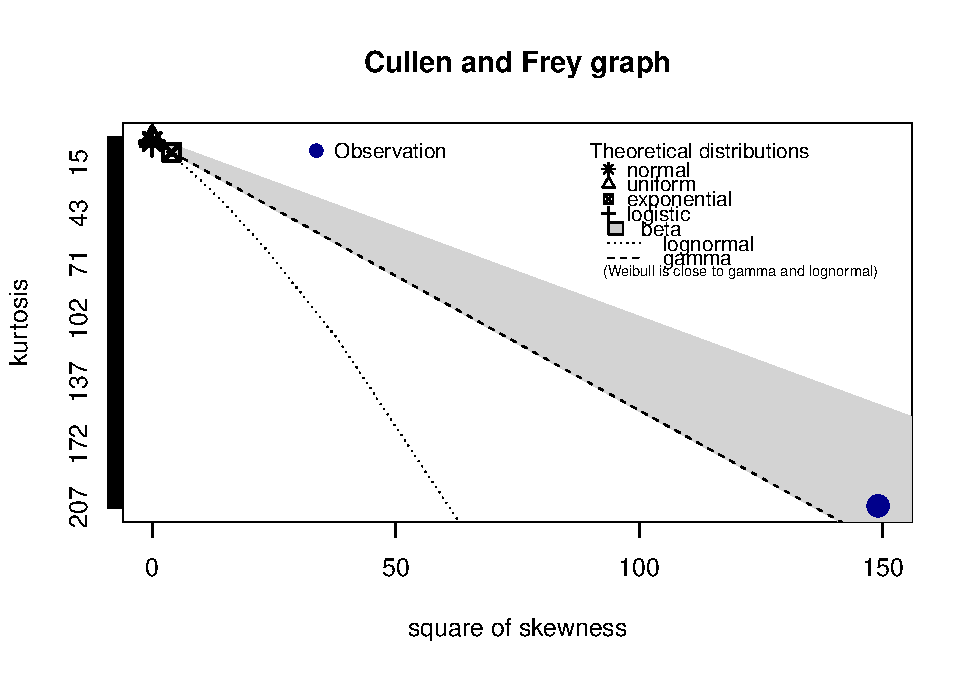
\includegraphics{Final_Project_files/figure-latex/unnamed-chunk-5-1.pdf}

\begin{verbatim}
## summary statistics
## ------
## min:  1300   max:  215245 
## median:  9478.5 
## mean:  10516.83 
## estimated sd:  9981.265 
## estimated skewness:  12.20769 
## estimated kurtosis:  206.2433
\end{verbatim}

\section{TODO figure out why beta distribution is not
working}\label{todo-figure-out-why-beta-distribution-is-not-working}

\begin{Shaded}
\begin{Highlighting}[]
\KeywordTok{library}\NormalTok{(MASS)}
\KeywordTok{fitdistr}\NormalTok{(}\KeywordTok{as.numeric}\NormalTok{(sub.train.df$LotArea), }\DataTypeTok{densfun =} \StringTok{"normal"}\NormalTok{)}
\end{Highlighting}
\end{Shaded}

\begin{verbatim}
##       mean          sd    
##   10516.8281    9977.8461 
##  (  261.1322) (  184.6483)
\end{verbatim}

Find the optimal value of the parameters for this distribution, and then
take 1000 samples from this distribution (e.g., rexp(1000) for an
exponential).

Plot a histogram and compare it with a histogram of your non-transformed
original variable.

\section{Modeling}\label{modeling}

Build some type of regression model and submit your model to the
competition board.

Provide your complete model summary and results with analysis.

Report your Kaggle.com user name and score.

Multiply the correlation matrix by the precision matrix, and then
multiply the precision matrix by the correlation matrix.


\end{document}
